
\subsection{Diseño}

La etapa de diseño fue de especial importancia, ya que tratandose del primer incremento sirvió para asentar aspectos generales del proyecto, tanto de estructuración y flujo de datos como de interfaz de usuario.

\subsubsection{Diseño de datos}
\label{c:diseño_datos}

Durante el diseño de datos se definieron dos aspectos fundamentales: la estructura y el flujo de datos.

\textbf{En primer lugar}, con respecto a la \textbf{estructura de datos}, se identificaron los datos mínimos indispensables tomando como referencia los objetivos y requisitos del incremento:

\begin{itemize}
    \item \textbf{Correo electrónico}, único y con el que el usuario podrá identificarse en la aplicación web.
    \item \textbf{Contraseña}, con un máximo de 6 carácteres.
    \item \textbf{Nombre de usuario}, único y con un tamaño máximo de 10 carácteres, con el que se diferenciará publicamente del resto de usuarios.
    \item \textbf{Descripción}, opcional y con un tamaño máximo de 150 carácteres, con el que el usuario podrá describirse brevemente.
\end{itemize}

A continuación se estudió el funcionamiento de \textit{Supabase}, el cual provee de un servicio de autenticación con su propia tabla predefinida. Se determinó utilizar la tabla facilitada por \textit{Supabase} para los perfiles privados y la creación de una nueva tabla con los datos restantes para el perfil público. Se estableció una relación entre ambas a través del identificador generado por \textit{Supabase} en la tabla del perfil privado \figref{fig:diagrama_datos_i1}.

\begin{figure}[H]
    \centering
    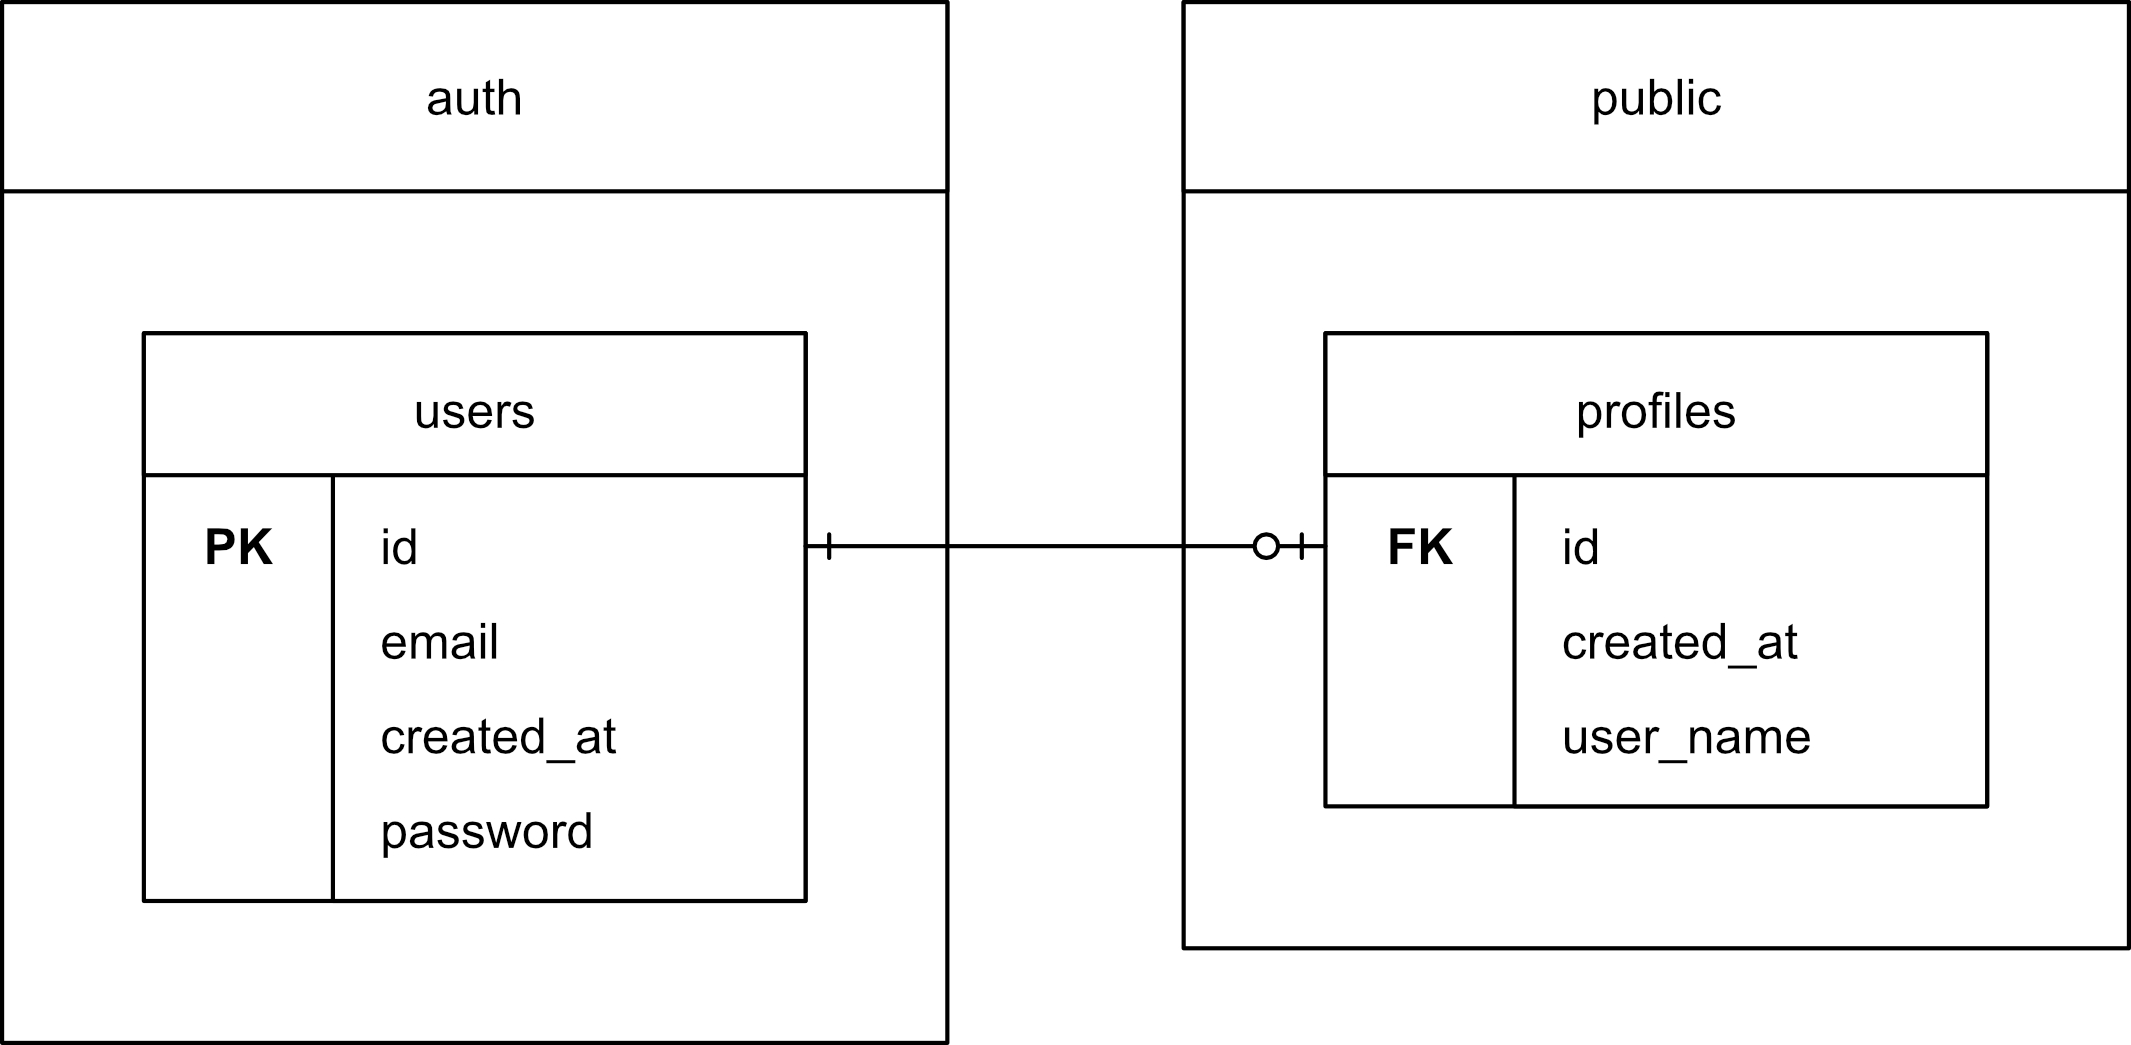
\includegraphics[width=0.6\textwidth]{Ilustraciones/desarrollo/incremento1/diagrama_datos_i1.jpg}
    \caption{Diagrama de estructura de datos de los perfiles de usuario}\label{fig:diagrama_datos_i1}
\end{figure}

\textbf{En segundo lugar}, con respecto al \textbf{flujo de datos}, y con el objetivo de garantizar la correcta comunicación de la información, se decidió emplear:

\begin{itemize}
    \item \textbf{Acciones desde el servidor}, priorizando su uso frente al manejo, transformación o consulta de datos desde el cliente.
    \item \textbf{Validadores}, para la verificación de datos, tales como tamaño \textit{(e.g. nombre de usuario, contraseña, descripción)} y formato \textit{(e.g. correo)}.
    \item \textbf{\textit{Data Transfer Object - DTO}}~\cite{wikipedia_dto}, a modo de interfaces para la definición de conjuntos de datos.
    \item \textbf{\textit{Mapeadores}}, para la transformación en conjuntos de datos basados en las interfaces \textit{DTO}.  
\end{itemize}

Los elementos anteriores fueron implementados según las necesidades de la consulta, sirviendo como proceso intermediario entre el cliente, el servidor y \textit{Supabase} \figref{fig:diagramas_flujo}.

\begin{figure}[H]
    \centering

    \begin{subfigure}[t]{0.4\textwidth}
        \centering
        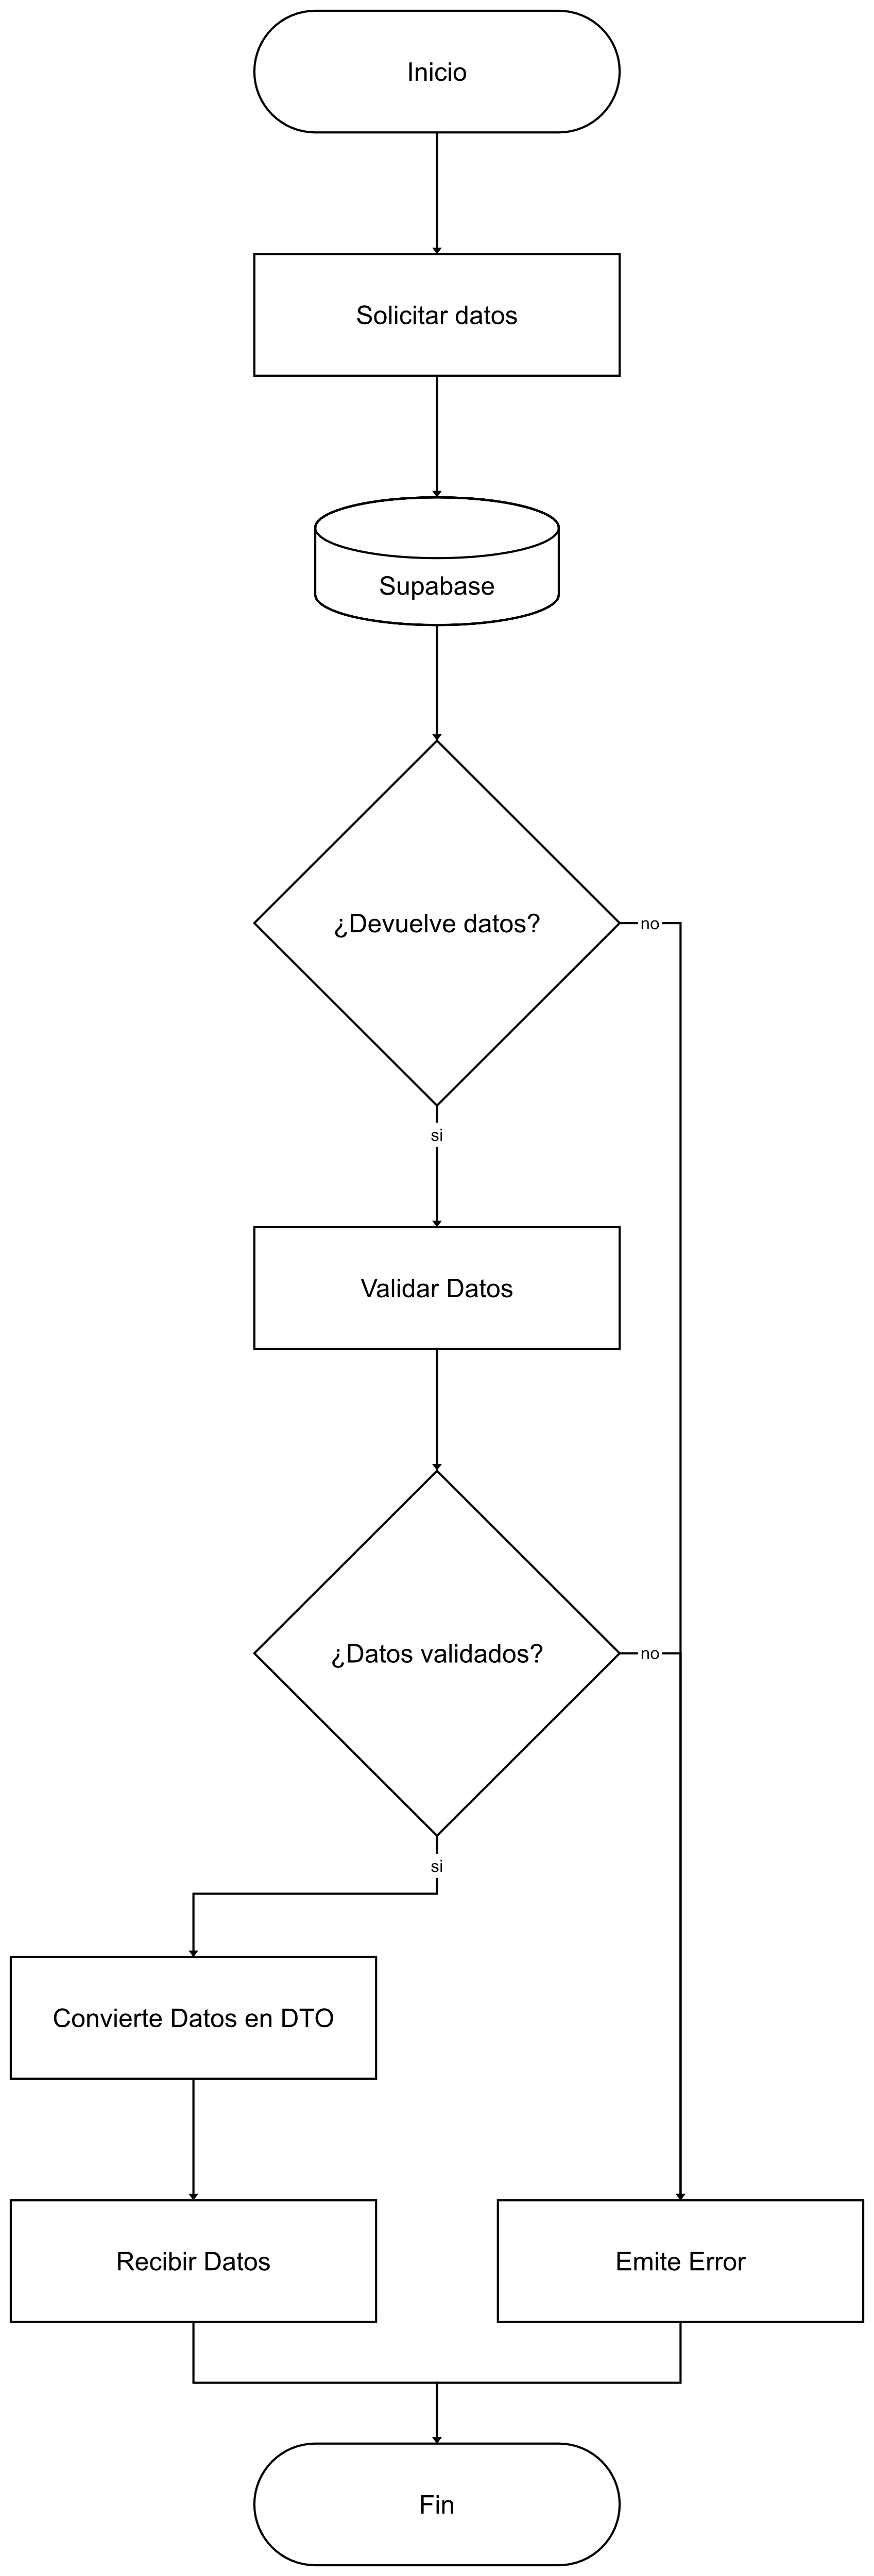
\includegraphics[width=\textwidth]{Ilustraciones/desarrollo/incremento1/diagrama_flujo_i1.jpg}
        \caption{Diagrama de flujo de datos de solicitud de información}\label{fig:diagrama_flujo_obtener}
    \end{subfigure}
    \hfill
    \begin{subfigure}[t]{0.3\textwidth}
        \centering
     
        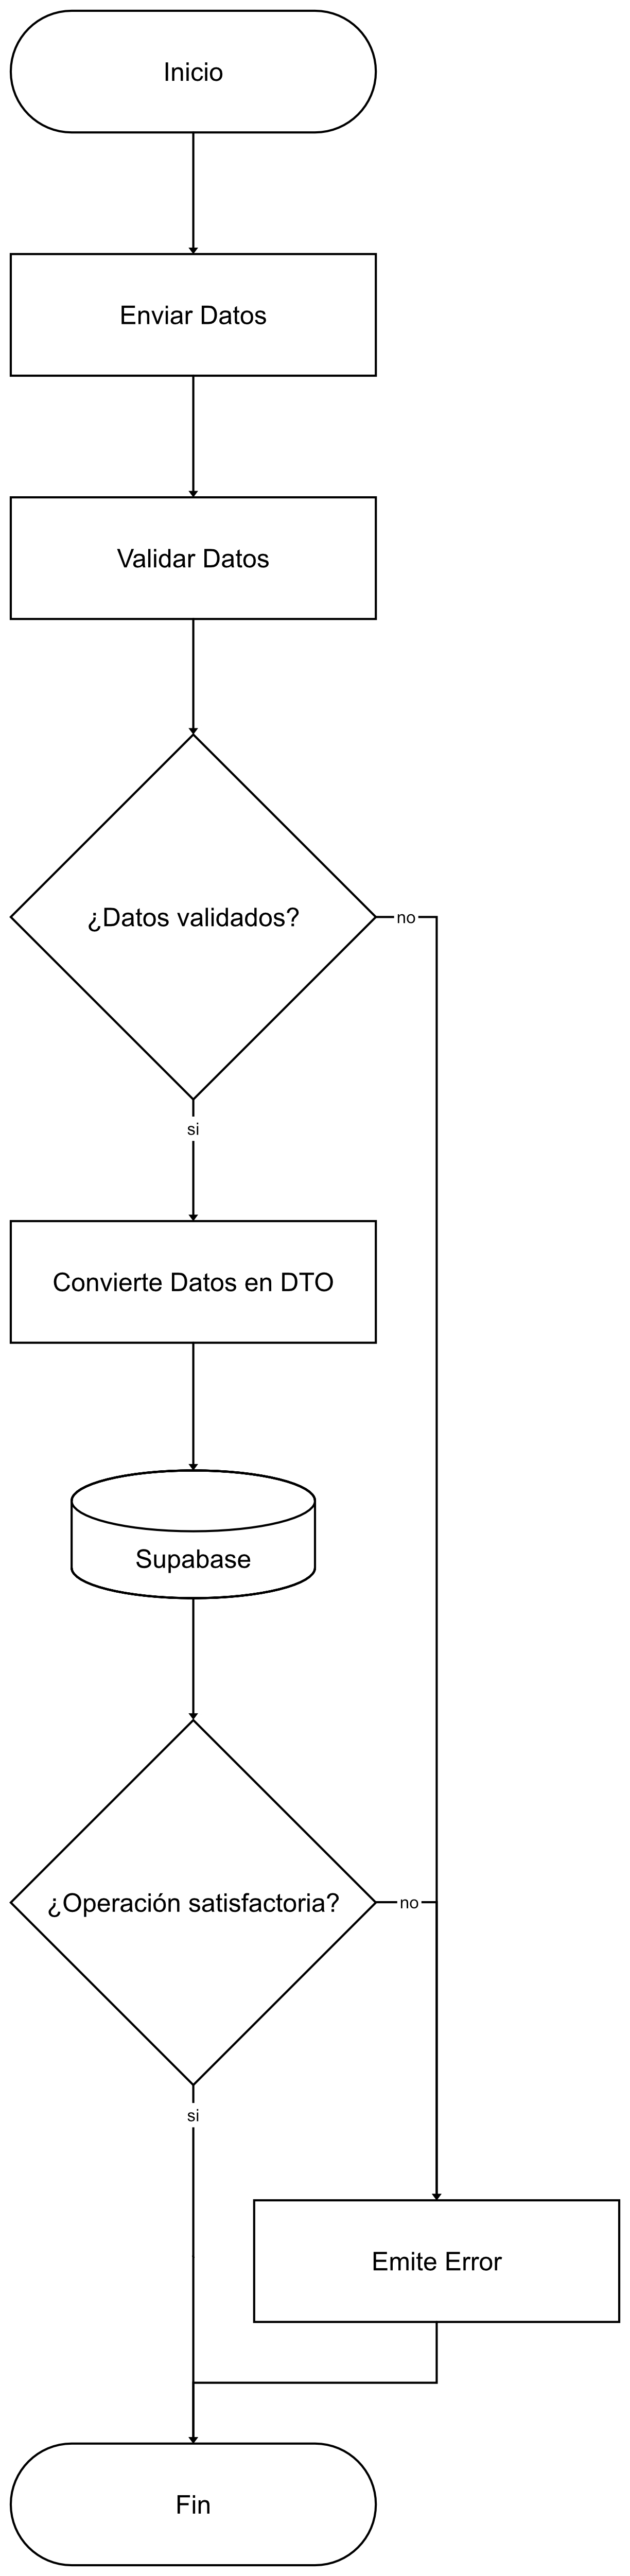
\includegraphics[width=\textwidth]{Ilustraciones/desarrollo/incremento1/diagrama_flujo2_i1.jpg}
        \caption{Diagrama de flujo de datos de modificación de información}\label{fig:diagrama_flujo_modificar}
    \end{subfigure}
    \caption{Páginas de LaCuerda.}
    \label{fig:diagramas_flujo}
\end{figure}


\subsubsection{Diseño de interfaz}
\label{c:diseño_interfaz}

Para el diseño de la interfaz se tomaron decisiones respecto a la utilización de colores, isologo, diseño de componentes comunes y páginas a desarrollar.

\textbf{En primer lugar}, se diseñó la paleta de colores \figref{fig:ui_palette} y su uso en distintos componentes de la interfaz \figref{fig:ui_guide}.

\begin{figure}[H]
    \centering
    \begin{subfigure}[t]{0.48\textwidth}
        \centering
        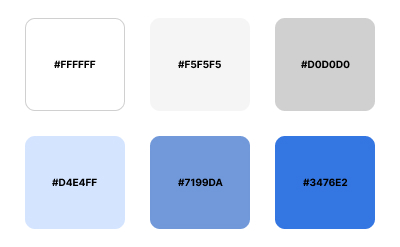
\includegraphics[width=1\textwidth]{Ilustraciones/desarrollo/incremento1/diseño/color_palette.jpg}
        \caption{Paleta de colores}\label{fig:ui_palette}
    \end{subfigure}
    \hfill
    \begin{subfigure}[t]{0.48\textwidth}
        \centering
        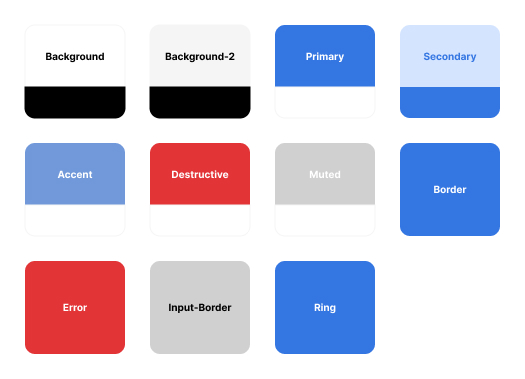
\includegraphics[width=\textwidth]{Ilustraciones/desarrollo/incremento1/diseño/color_scheme.jpg}
        \caption{Guía de colores}\label{fig:ui_guide}
    \end{subfigure}\caption{Colores utilizados en la interfaz}\label{fig:ui_colors}
\end{figure}

\textbf{En segundo lugar}, se diseñó el isologo de la aplicación web \figref{fig:ui_logo}, el cual combina el timple con el nombre de la aplicación web \textbf{Timple Tabs}.

\begin{figure}[H]
    \centering
    
\includegraphics[width=0.4\textwidth]{Ilustraciones/desarrollo/incremento1/diseño/logo_2.png}
    \caption{Isologo de la aplicación web}\label{fig:ui_logo}
\end{figure}



\textbf{En tercer lugar}, se diseñaron los componentes comunes de la interfaz de usuario, tales como botones \figref{fig:ui_buttons}, campos de formulario \figref{fig:ui_fields}, diálogos \figref{fig:dialog}, información desplegable \figref{fig:dropdown_info}.

\begin{figure}[H]
    \centering
    \begin{subfigure}[t]{0.48\textwidth}
        \centering
        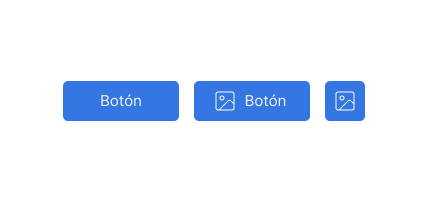
\includegraphics[width=1\textwidth]{Ilustraciones/desarrollo/incremento1/diseño/buttons.jpg}
        \caption{Botones y sus variantes según espacio}\label{fig:ui_buttons_variants}
    \end{subfigure}
    \hfill
    \begin{subfigure}[t]{0.48\textwidth}
        \centering
        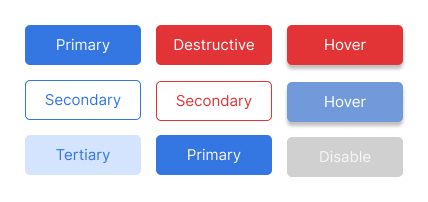
\includegraphics[width=1\textwidth]{Ilustraciones/desarrollo/incremento1/diseño/button_color_scheme.jpg}
        \caption{Botones y sus variantes según función y estado}\label{fig:ui_buttons_color}
    \end{subfigure}
    \vspace{1em}
    \begin{subfigure}[t]{\textwidth}{
        \centering
        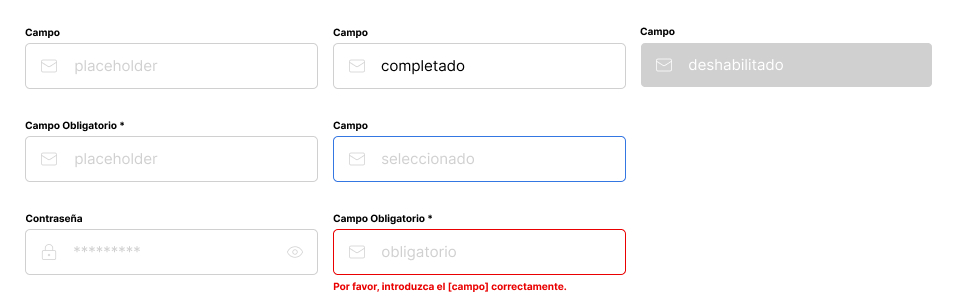
\includegraphics[width=\textwidth]{Ilustraciones/desarrollo/incremento1/diseño/fields.jpg}
        \caption{Campos y sus variantes según función y estado}\label{fig:ui_fields}}    
    \end{subfigure}
    \vspace{1em}
    \begin{subfigure}[t]{0.34\textwidth}
        \centering
        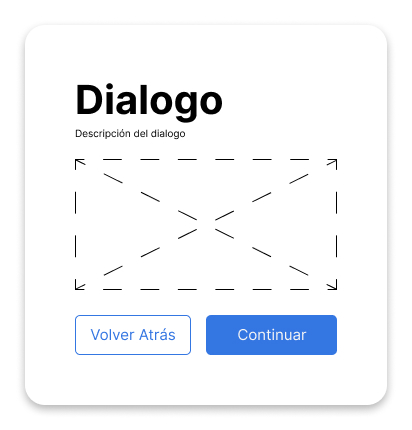
\includegraphics[width=1\textwidth]{Ilustraciones/desarrollo/incremento1/diseño/dialog.jpg}
        \caption{Dialogo sin contenido}\label{fig:dialog}
    \end{subfigure}
    \hfill
    \begin{subfigure}[t]{0.62\textwidth}
        \centering
        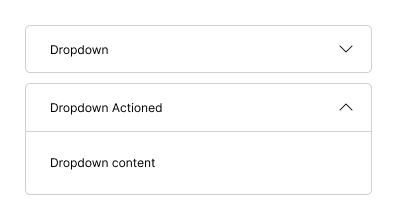
\includegraphics[width=1\textwidth]{Ilustraciones/desarrollo/incremento1/diseño/dropdown_info.jpg}
        \caption{Información desplegable}\label{fig:dropdown_info}
    \end{subfigure}
    
    \caption{Diseño de componentes comunes}\label{fig:ui_buttons}
\end{figure}

\textbf{Finalmente}, se realizó el diseño de las páginas correspondientes a la página principal \figref{fig:ui_home}, inicio de sesión \figref{fig:ui_login}, recuperación de contraseña \figref{fig:passrec}, registro \figref{fig:ui_register_empty}, perfil \figref{fig:ui_profile} y ajustes de cuenta \figref{fig:ui_settings}, utilizando el enfoque de diseño \textit{mobile-first} asegurando la correcta visualización y usabilidad en dispositivos moviles.

\begin{figure}[H]
    \centering
    \begin{subfigure}[t]{0.2\textwidth}
        \centering
        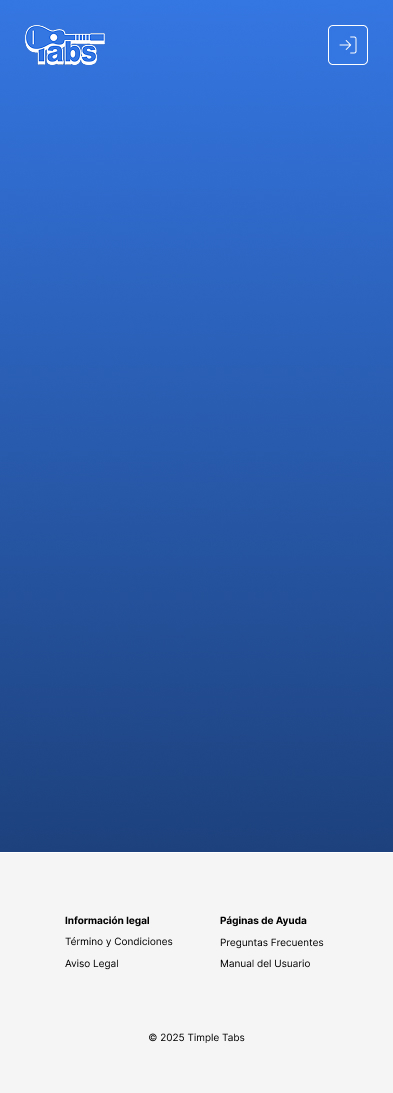
\includegraphics[width=1\textwidth]{Ilustraciones/desarrollo/incremento1/diseño/home_unregistered.jpg}
        \caption{Diseño de página principal de usuarios no registrados}\label{fig:ui_home}
    \end{subfigure}
    \hfill
    \begin{subfigure}[t]{0.2\textwidth}
        \centering
        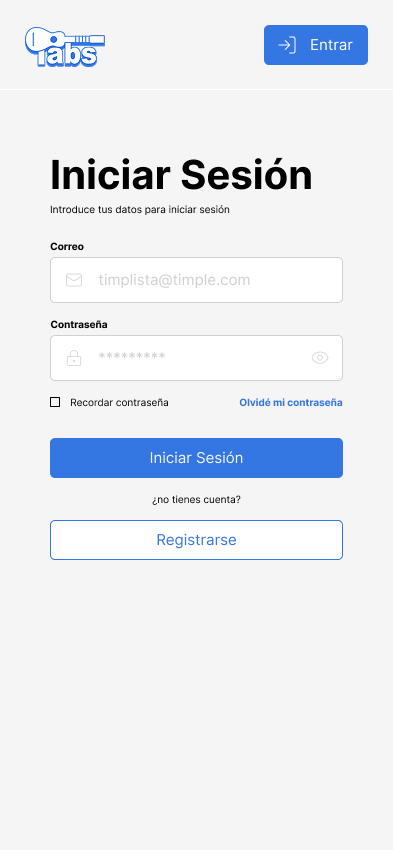
\includegraphics[width=1\textwidth]{Ilustraciones/desarrollo/incremento1/diseño/login.jpg}
        \caption{Diseño de página de inicio de sesión}\label{fig:ui_login}
    \end{subfigure}
    \hfill
    \begin{subfigure}[t]{0.2\textwidth}
        \centering
        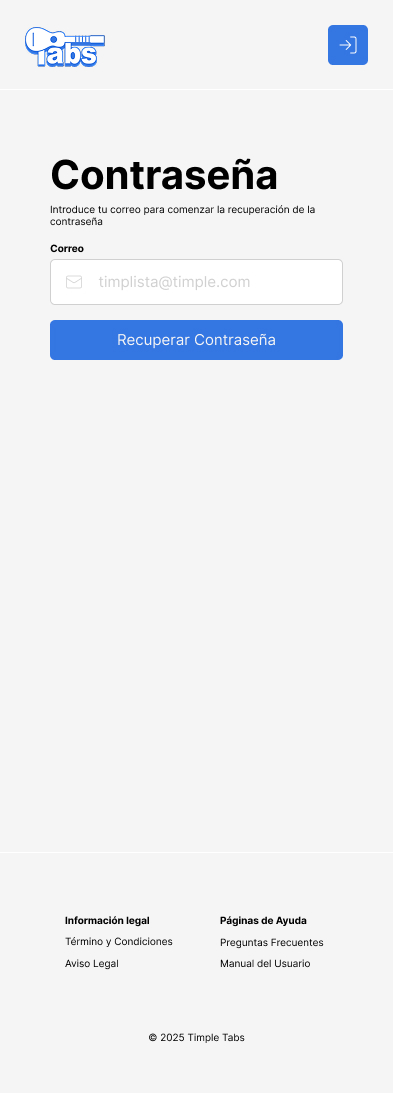
\includegraphics[width=1\textwidth]{Ilustraciones/desarrollo/incremento1/diseño/password_recovery.jpg}
        \caption{Diseño de página de recuperación de contraseña}\label{fig:passrec}
    \end{subfigure}
    \hfill
    \begin{subfigure}[t]{0.2\textwidth}
        \centering
        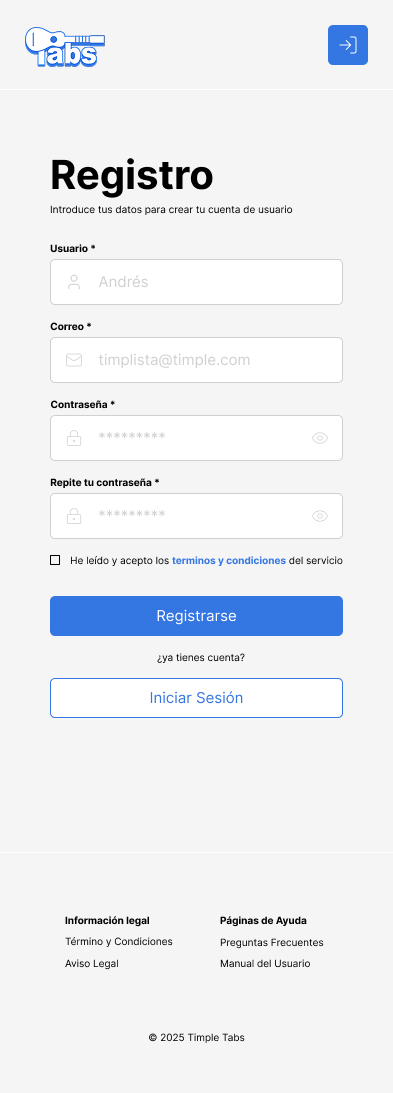
\includegraphics[width=1\textwidth]{Ilustraciones/desarrollo/incremento1/diseño/register.jpg}
        \caption{Diseño de pantalla de registro de usuario con campos vacios}\label{fig:ui_register_empty}
    \end{subfigure}
    \hfill
    \begin{subfigure}[t]{0.2\textwidth}
        \centering
        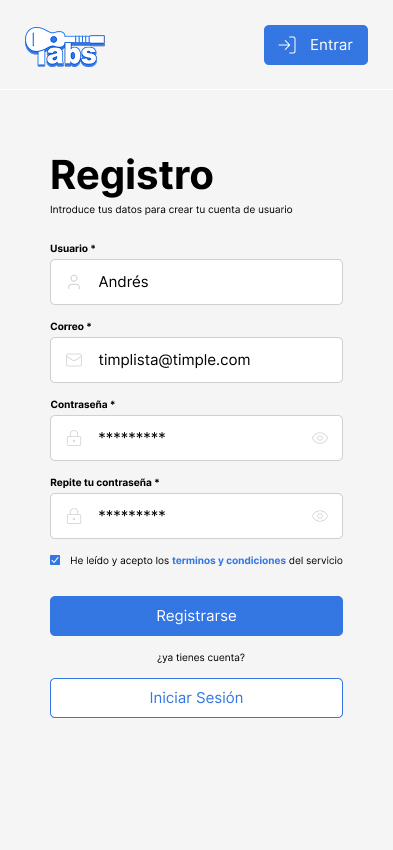
\includegraphics[width=1\textwidth]{Ilustraciones/desarrollo/incremento1/diseño/register_filled.jpg}
        \caption{Diseño de pantalla de registro de usuario con campos completados}\label{fig:ui_register_fill}
    \end{subfigure}
    \hfill
    \begin{subfigure}[t]{0.2\textwidth}
        \centering
        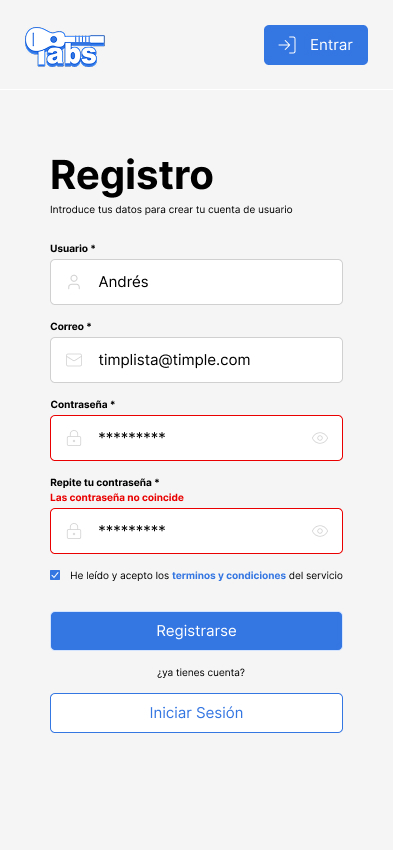
\includegraphics[width=1\textwidth]{Ilustraciones/desarrollo/incremento1/diseño/register_error.jpg}
        \caption{Diseño de pantalla de registro de usuario con campos incorrectos}\label{fig:ui_register_fail}
    \end{subfigure}
    \hfill
    \begin{subfigure}[t]{0.2\textwidth}
        \centering
        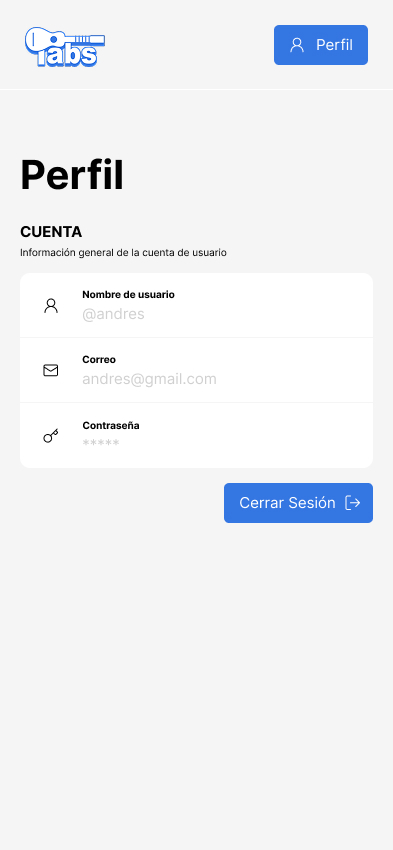
\includegraphics[width=1\textwidth]{Ilustraciones/desarrollo/incremento1/diseño/profile.jpg}
        \caption{Diseño de página de perfil de usuario}\label{fig:ui_profile}
    \end{subfigure}
    \hfill
    \begin{subfigure}[t]{0.2\textwidth}
        \centering
        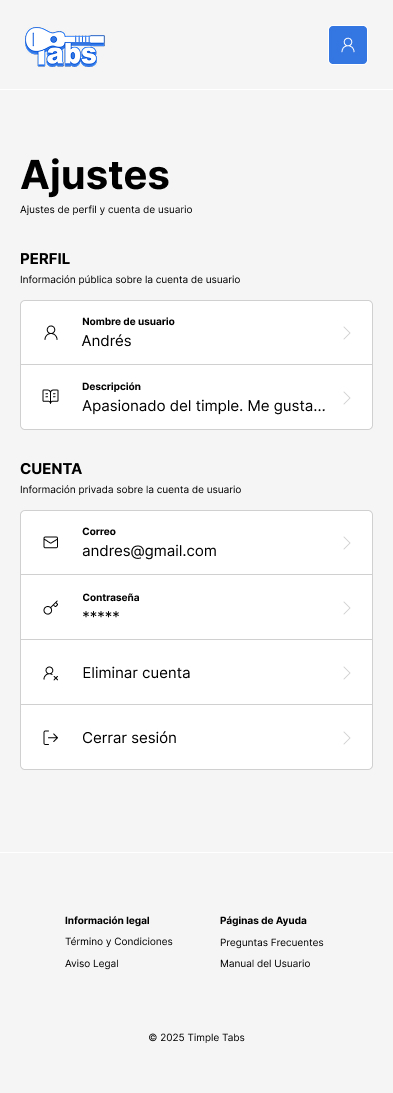
\includegraphics[width=1\textwidth]{Ilustraciones/desarrollo/incremento1/diseño/settings.jpg}
        \caption{Diseño de página de perfil de usuario}\label{fig:ui_settings}
    \end{subfigure}
    \vspace{1em}
    \caption{Diseño de página de ajustes de cuenta de usuario}\label{fig:ui_smt}
\end{figure}

Además, con el fín de garantizar la responsividad del diseño a distintas pantallas, se tradujo el diseño de las páginas anteriores a pantallas de mayor tamaño \figref{fig:ui_login_desktop}.

\begin{figure}[H]
    \centering
    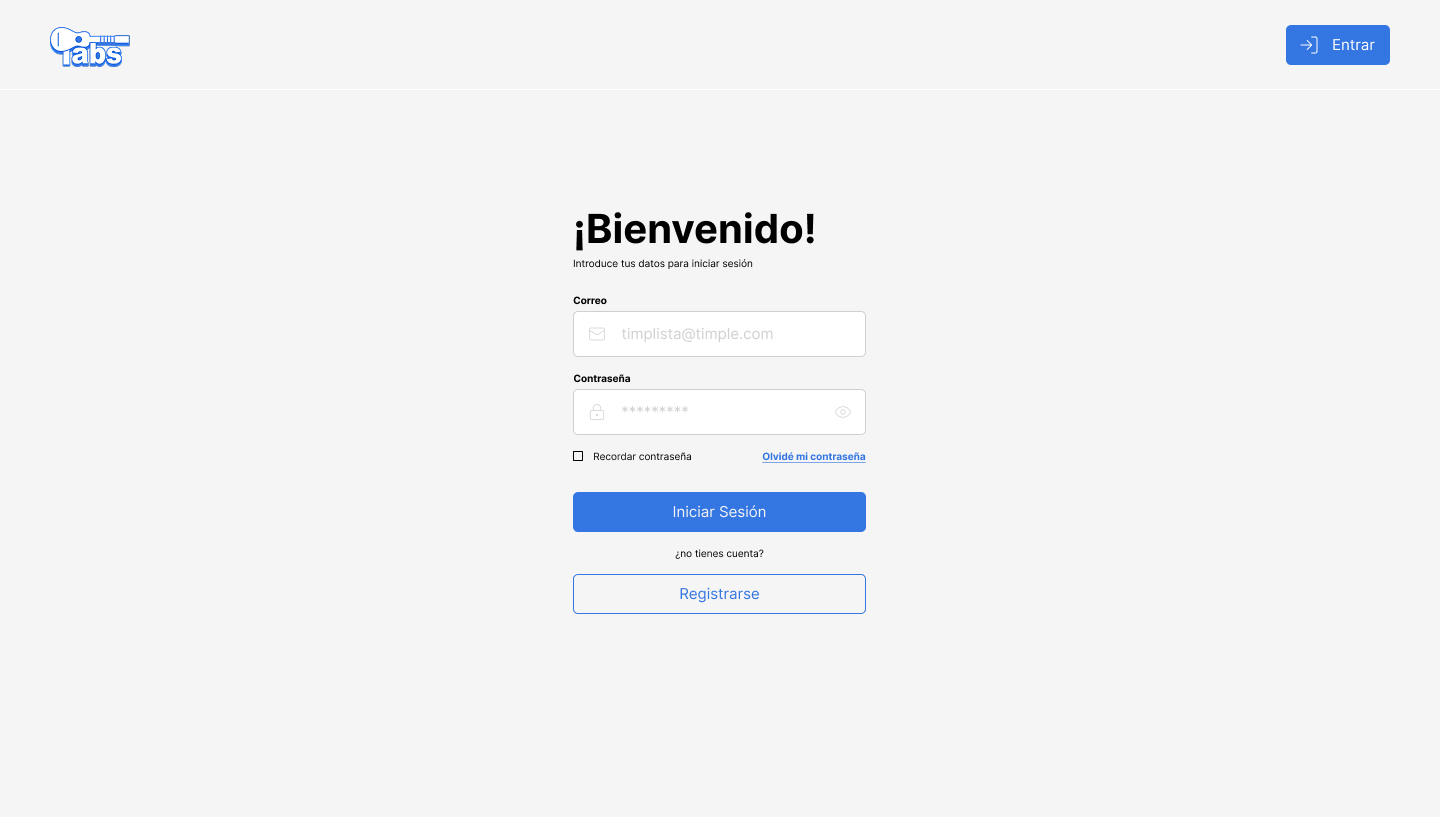
\includegraphics[width=0.8\textwidth]{Ilustraciones/desarrollo/incremento1/diseño/login_big.jpg}
    \caption{Diseño de página de inicio de sesión en pantalla grande}\label{fig:ui_login_desktop}
\end{figure}